\documentclass{standalone}
\usepackage{tikz}
\usetikzlibrary{patterns, positioning}


\begin{document}
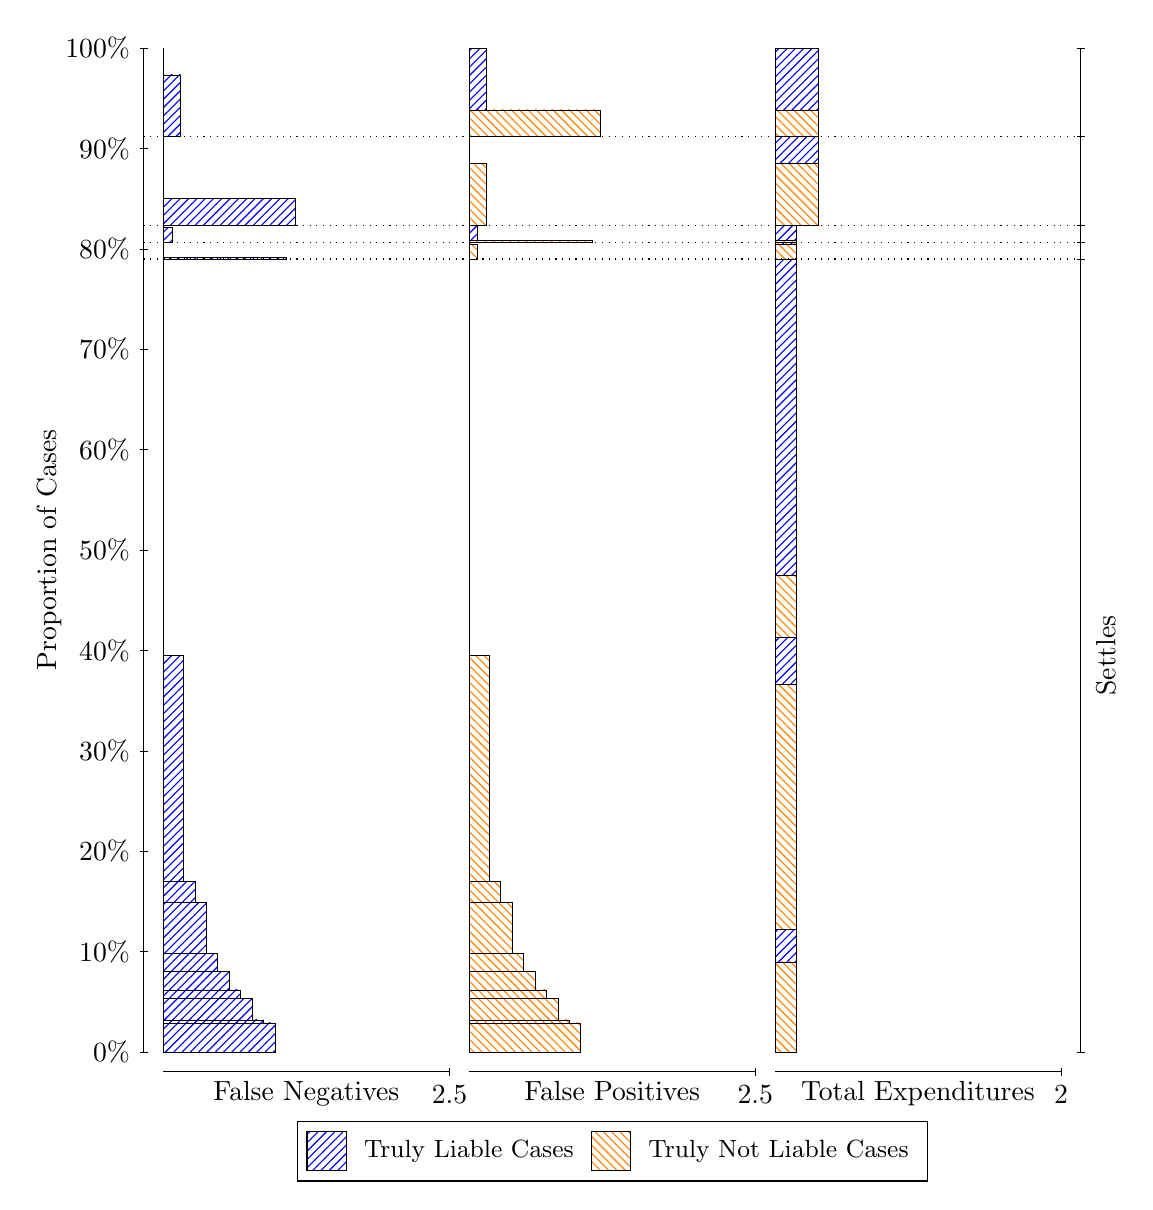
\begin{tikzpicture}
\draw[black, very thin] (1.5,1.75) -- (1.5,14.5);
\node[rotate=90, text=black, anchor=center] at (0.3, 8.125) {Proportion of Cases};
\draw[black, very thin] (1.45,1.75) -- (1.55,1.75);
\node[text=black, anchor=east] at (1.45, 1.75) {0\%};
\draw[black, very thin] (1.45,3.025) -- (1.55,3.025);
\node[text=black, anchor=east] at (1.45, 3.025) {10\%};
\draw[black, very thin] (1.45,4.3) -- (1.55,4.3);
\node[text=black, anchor=east] at (1.45, 4.3) {20\%};
\draw[black, very thin] (1.45,5.575) -- (1.55,5.575);
\node[text=black, anchor=east] at (1.45, 5.575) {30\%};
\draw[black, very thin] (1.45,6.85) -- (1.55,6.85);
\node[text=black, anchor=east] at (1.45, 6.85) {40\%};
\draw[black, very thin] (1.45,8.125) -- (1.55,8.125);
\node[text=black, anchor=east] at (1.45, 8.125) {50\%};
\draw[black, very thin] (1.45,9.4) -- (1.55,9.4);
\node[text=black, anchor=east] at (1.45, 9.4) {60\%};
\draw[black, very thin] (1.45,10.675) -- (1.55,10.675);
\node[text=black, anchor=east] at (1.45, 10.675) {70\%};
\draw[black, very thin] (1.45,11.95) -- (1.55,11.95);
\node[text=black, anchor=east] at (1.45, 11.95) {80\%};
\draw[black, very thin] (1.45,13.225) -- (1.55,13.225);
\node[text=black, anchor=east] at (1.45, 13.225) {90\%};
\draw[black, very thin] (1.45,14.5) -- (1.55,14.5);
\node[text=black, anchor=east] at (1.45, 14.5) {100\%};

\draw[black, very thin] (13.4,1.75) -- (13.4,14.5);
\draw[black, very thin] (13.35,1.75) -- (13.45,1.75);
\node[anchor=west] at (13.35, 1.75) {};
\draw[black, very thin] (13.35,11.821) -- (13.45,11.821);
\node[anchor=west] at (13.35, 11.821) {};
\draw[black, very thin] (13.35,12.034) -- (13.45,12.034);
\node[anchor=west] at (13.35, 12.034) {};
\draw[black, very thin] (13.35,12.246) -- (13.45,12.246);
\node[anchor=west] at (13.35, 12.246) {};
\draw[black, very thin] (13.35,13.373) -- (13.45,13.373);
\node[anchor=west] at (13.35, 13.373) {};
\draw[black, very thin] (13.35,14.5) -- (13.45,14.5);
\node[anchor=west] at (13.35, 14.5) {};

\draw[black, very thin, pattern color=blue, pattern=north east lines] (1.75,1.75) rectangle (3.167,2.1199);
\draw[black, very thin, pattern color=blue, pattern=north east lines] (1.75,2.1199) rectangle (3.0217,2.1562);
\draw[black, very thin, pattern color=blue, pattern=north east lines] (1.75,2.1562) rectangle (2.8763,2.4354);
\draw[black, very thin, pattern color=blue, pattern=north east lines] (1.75,2.4354) rectangle (2.731,2.5386);
\draw[black, very thin, pattern color=blue, pattern=north east lines] (1.75,2.5386) rectangle (2.5857,2.7721);
\draw[black, very thin, pattern color=blue, pattern=north east lines] (1.75,2.7721) rectangle (2.4403,2.9982);
\draw[black, very thin, pattern color=blue, pattern=north east lines] (1.75,2.9982) rectangle (2.295,3.6497);
\draw[black, very thin, pattern color=blue, pattern=north east lines] (1.75,3.6497) rectangle (2.1497,3.9152);
\draw[black, very thin, pattern color=blue, pattern=north east lines] (1.75,3.9152) rectangle (2.0043,6.7857);
\draw[black, very thin, pattern color=orange, pattern=north west lines] (1.75,6.7857) rectangle (1.75,11.821);
\draw[black, very thin, pattern color=blue, pattern=north east lines] (1.75,11.821) rectangle (3.3123,11.842);
\draw[black, very thin, pattern color=orange, pattern=north west lines] (1.75,11.842) rectangle (1.75,12.034);
\draw[black, very thin, pattern color=blue, pattern=north east lines] (1.75,12.034) rectangle (1.859,12.225);
\draw[black, very thin, pattern color=orange, pattern=north west lines] (1.75,12.225) rectangle (1.75,12.246);
\draw[black, very thin, pattern color=blue, pattern=north east lines] (1.75,12.246) rectangle (3.4213,12.588);
\draw[black, very thin, pattern color=orange, pattern=north west lines] (1.75,12.588) rectangle (1.75,13.373);
\draw[black, very thin, pattern color=blue, pattern=north east lines] (1.75,13.373) rectangle (1.968,14.158);
\draw[black, very thin, pattern color=orange, pattern=north west lines] (1.75,14.158) rectangle (1.75,14.5);
\draw[black, very thin, pattern color=orange, pattern=north west lines] (5.6333,1.75) rectangle (7.0503,2.1199);
\draw[black, very thin, pattern color=orange, pattern=north west lines] (5.6333,2.1199) rectangle (6.905,2.1562);
\draw[black, very thin, pattern color=orange, pattern=north west lines] (5.6333,2.1562) rectangle (6.7597,2.4353);
\draw[black, very thin, pattern color=orange, pattern=north west lines] (5.6333,2.4353) rectangle (6.6143,2.5386);
\draw[black, very thin, pattern color=orange, pattern=north west lines] (5.6333,2.5386) rectangle (6.469,2.7721);
\draw[black, very thin, pattern color=orange, pattern=north west lines] (5.6333,2.7721) rectangle (6.3237,2.9982);
\draw[black, very thin, pattern color=orange, pattern=north west lines] (5.6333,2.9982) rectangle (6.1783,3.6497);
\draw[black, very thin, pattern color=orange, pattern=north west lines] (5.6333,3.6497) rectangle (6.033,3.9152);
\draw[black, very thin, pattern color=orange, pattern=north west lines] (5.6333,3.9152) rectangle (5.8877,6.7858);
\draw[black, very thin, pattern color=blue, pattern=north east lines] (5.6333,6.7858) rectangle (5.6333,11.821);
\draw[black, very thin, pattern color=orange, pattern=north west lines] (5.6333,11.821) rectangle (5.7423,12.013);
\draw[black, very thin, pattern color=blue, pattern=north east lines] (5.6333,12.013) rectangle (5.6333,12.034);
\draw[black, very thin, pattern color=orange, pattern=north west lines] (5.6333,12.034) rectangle (7.1957,12.054);
\draw[black, very thin, pattern color=blue, pattern=north east lines] (5.6333,12.054) rectangle (5.7423,12.246);
\draw[black, very thin, pattern color=orange, pattern=north west lines] (5.6333,12.246) rectangle (5.8513,13.031);
\draw[black, very thin, pattern color=blue, pattern=north east lines] (5.6333,13.031) rectangle (5.6333,13.373);
\draw[black, very thin, pattern color=orange, pattern=north west lines] (5.6333,13.373) rectangle (7.3047,13.715);
\draw[black, very thin, pattern color=blue, pattern=north east lines] (5.6333,13.715) rectangle (5.8513,14.5);
\draw[black, very thin, pattern color=orange, pattern=north west lines] (9.5167,1.75) rectangle (9.7892,2.8931);
\draw[black, very thin, pattern color=blue, pattern=north east lines] (9.5167,2.8931) rectangle (9.7892,3.3117);
\draw[black, very thin, pattern color=orange, pattern=north west lines] (9.5167,3.3117) rectangle (9.7892,6.4159);
\draw[black, very thin, pattern color=blue, pattern=north east lines] (9.5167,6.4159) rectangle (9.7892,7.0194);
\draw[black, very thin, pattern color=orange, pattern=north west lines] (9.5167,7.0194) rectangle (9.7892,7.808);
\draw[black, very thin, pattern color=blue, pattern=north east lines] (9.5167,7.808) rectangle (9.7892,11.821);
\draw[black, very thin, pattern color=orange, pattern=north west lines] (9.5167,11.821) rectangle (9.7892,12.013);
\draw[black, very thin, pattern color=blue, pattern=north east lines] (9.5167,12.013) rectangle (9.7892,12.034);
\draw[black, very thin, pattern color=orange, pattern=north west lines] (9.5167,12.034) rectangle (9.7892,12.054);
\draw[black, very thin, pattern color=blue, pattern=north east lines] (9.5167,12.054) rectangle (9.7892,12.246);
\draw[black, very thin, pattern color=orange, pattern=north west lines] (9.5167,12.246) rectangle (10.062,13.031);
\draw[black, very thin, pattern color=blue, pattern=north east lines] (9.5167,13.031) rectangle (10.062,13.373);
\draw[black, very thin, pattern color=orange, pattern=north west lines] (9.5167,13.373) rectangle (10.062,13.715);
\draw[black, very thin, pattern color=blue, pattern=north east lines] (9.5167,13.715) rectangle (10.062,14.5);
\draw[black, dotted] (1.5,11.821) -- (13.4,11.821);
\draw[black, dotted] (1.5,12.034) -- (13.4,12.034);
\draw[black, dotted] (1.5,12.246) -- (13.4,12.246);
\draw[black, dotted] (1.5,13.373) -- (13.4,13.373);
\draw[black, very thin] (1.75,1.5) -- (5.3833,1.5);
\node[text=black, anchor=north] at (3.5667, 1.5) {False Negatives};
\draw[black, very thin] (5.3833,1.45) -- (5.3833,1.55);
\node[text=black, anchor=north] at (5.3833, 1.45) {2.5};

\draw[black, very thin] (5.6333,1.5) -- (9.2667,1.5);
\node[text=black, anchor=north] at (7.45, 1.5) {False Positives};
\draw[black, very thin] (9.2667,1.45) -- (9.2667,1.55);
\node[text=black, anchor=north] at (9.2667, 1.45) {2.5};

\draw[black, very thin] (9.5167,1.5) -- (13.15,1.5);
\node[text=black, anchor=north] at (11.333, 1.5) {Total Expenditures};
\draw[black, very thin] (13.15,1.45) -- (13.15,1.55);
\node[text=black, anchor=north] at (13.15, 1.45) {2};

\node[text=black, centered, rotate=90] at (13.72, 6.7857) {Settles};





\draw (7.449999999999999,1.5) node[draw=none] (baseCoordinate) {};
\begin{scope}[align=center]
        \matrix[scale=0.5, draw=black, below=0.5cm of baseCoordinate, nodes={draw}, column sep=0.1cm]{
            \node[rectangle, draw, minimum width=0.5cm, minimum height=0.5cm, pattern color=blue, pattern=north east lines] {}; &
            \node[draw=none, font=\small, text=black] (B) {Truly Liable Cases}; &
            \node[rectangle, draw, minimum width=0.5cm, minimum height=0.5cm, pattern color=orange, pattern=north west lines] {}; &
            \node[draw=none, font=\small, text=black] (B) {Truly Not Liable Cases}; \\
            };
\end{scope}

\end{tikzpicture}
\end{document}